% poster-exemplo (versão minimalista)
% http://www.vision.ime.usp.br/~jmena/stuff/poster-exemplo/
%
% Sáb Nov 12 16:20:02 BRST 2011
%
% OBSERVAÇÕES:
%  - Este exemplo de poster foi adaptado (em 08/2010) considerando os modelos:
%    (a) https://teamwork.jacobs-university.de:8443/confluence/display/CoPandBiG/LaTeX+Poster
%    (b) http://www.nathanieljohnston.com/2009/08/latex-poster-template/
%
%  - Veja as dimensões dos posters em: 
%    http://www.theinternetprinter.com.au/info/A4_A3_A2_A1_A0_Size_Explained.aspx
%

\documentclass[final]{beamer} 
\usepackage[size=a1, orientation=portrait]{beamerposter} % font scale factor=1.0

\usepackage[brazilian]{babel}
\usepackage[utf8]{inputenc}

% cores utilizadas para os algoritmos
\usepackage{framed}
\definecolor{treinamento}{rgb}{0.76471,0.81176,0.91373}  % c3cfe9 -> 195,207,233 -> 0.76471   0.81176   0.91373
\definecolor{reconstrucao}{rgb}{0.83529,0.80784,0.89804} % d5cee5 -> 213,206,229 -> 0.83529   0.80784   0.89804

\graphicspath{{./figures/}}  
\urlstyle{same}

%==The poster style============================================================
\usetheme{poster-exemplo}            % our poster style
%--set colors for blocks (without frame)---------------------------------------
  \setbeamercolor{block title}{fg=ngreen,bg=white}
  \setbeamercolor{block body}{fg=black,bg=white}
%--set colors for alerted blocks (with frame)----------------------------------
%--textcolor = fg, backgroundcolor = bg, dblue is the jacobs blue
  \setbeamercolor{block alerted title}{fg=white,bg=dblue!70}%frame color
  \setbeamercolor{block alerted body}{fg=black,bg=dblue!10}%body color
%
%==Titel, date and authors of the poster=======================================
\title{MatrUSP: Combinador de Grades Horárias para a USP \\ \url{http://bcc.ime.usp.br/matrusp}}
\author{Pedro Paulo Vezzá Campos}
\institute{Projeto Apoio BCC -- Instituto de Matemática e Estatística -- 
Universidade de São Paulo}
\date{\today}


%==============================================================================
%==the poster content==========================================================
%==============================================================================
\begin{document}
%--the poster is one beamer frame, so we have to start with:
\begin{frame}[t]
%--to seperate the poster in columns we can use the columns environment
\begin{columns}[t] % the [t] options aligns the columns content at the top
%--the left column-------------------------------------------------------------
%\begin{column}{0.28\paperwidth}% the right size for a 3-column layout
\begin{column}{0.35\paperwidth}% the right size for a 3-column layout

	\begin{alertblock}{Introdução}
		Semestralmente quase \textbf{60.000 alunos de graduação da USP} \cite{usp_numeros} devem montar suas
		grades horárias para o próximo semestre, escolhendo quais disciplinas
		pretendem cursar e em quais turmas. Esse processo de montagem atualmente
		é feito em sua maior parte manualmente pelo aluno. Ele acessa o sistema
		JupiterWeb em busca das turmas e horários disponíveis tentando encaixar
		as disciplinas para montar sua grade.
		
		\vskip2ex
		
		Com isso, diversos problemas surgem: Graduações com grandes quantidades de
		alunos tendem a ter diversas turmas possíveis e \textbf{achar uma combinação
		satisfatória pode demorar bastante tempo}, algo similar acontece com alunos
		em processo de escolha de disciplinas optativas.
		
		\vskip2ex
		
		O MatrUSP visa resolver esse problema fornecendo um \textbf{sistema simples} no
		qual o aluno indica apenas quais matérias deseja cursar e o programa apresenta
		todas as \textbf{combinações viáveis} de horários de uma \textbf{maneira visual e bastante
		intuitiva} ao aluno que pode proceder com a sua matrícula de maneira tradicional.
		
		\vskip2ex
		
		O projeto visa a simplicidade sendo uma ferramenta de uso único e simples
		de ser utilizada. Ainda, há o respeito pelas informações pessoais do usuário,
		o MatrUSP pode ser utilizado sem a necessidade de fornecer quaisquer identificações
		desnecessárias ao seu funcionamento.
		
	\end{alertblock}

\end{column}

% ---------------------------------------------------------------------------- %
\begin{column}{0.60\paperwidth} 
	\begin{block}{Trabalhos Relacionados}
		\begin{columns}[totalwidth=0.60\paperwidth]
		\begin{column}{0.28\paperwidth}
		O \textbf{MatrUFSC} \cite{matrufsc} surgiu como o sucessor do sistema GRAMA (GRAde de 
		MAtrícula) para a tarefa de montagem de grades de horários após o GRAMA,
		já tecnologicamente defasado, ter perdido o apoio da UFSC quando o autor
		tentou se aproveitar da popularidade do serviço para fazer propaganda
		própria da empresa criada pelo seu autor, que acabara de se formar da UFSC.

		\vskip2ex

		O MatrUSP surgiu como uma adaptação autorizada do MatrUFSC, através da
		liberação do seu código fonte pelo seu desenvolvedor, Ramiro Polla, 
		para o desenvolvimento do MatrUSP.
		
		\vskip2ex
		
		\begin{center}
			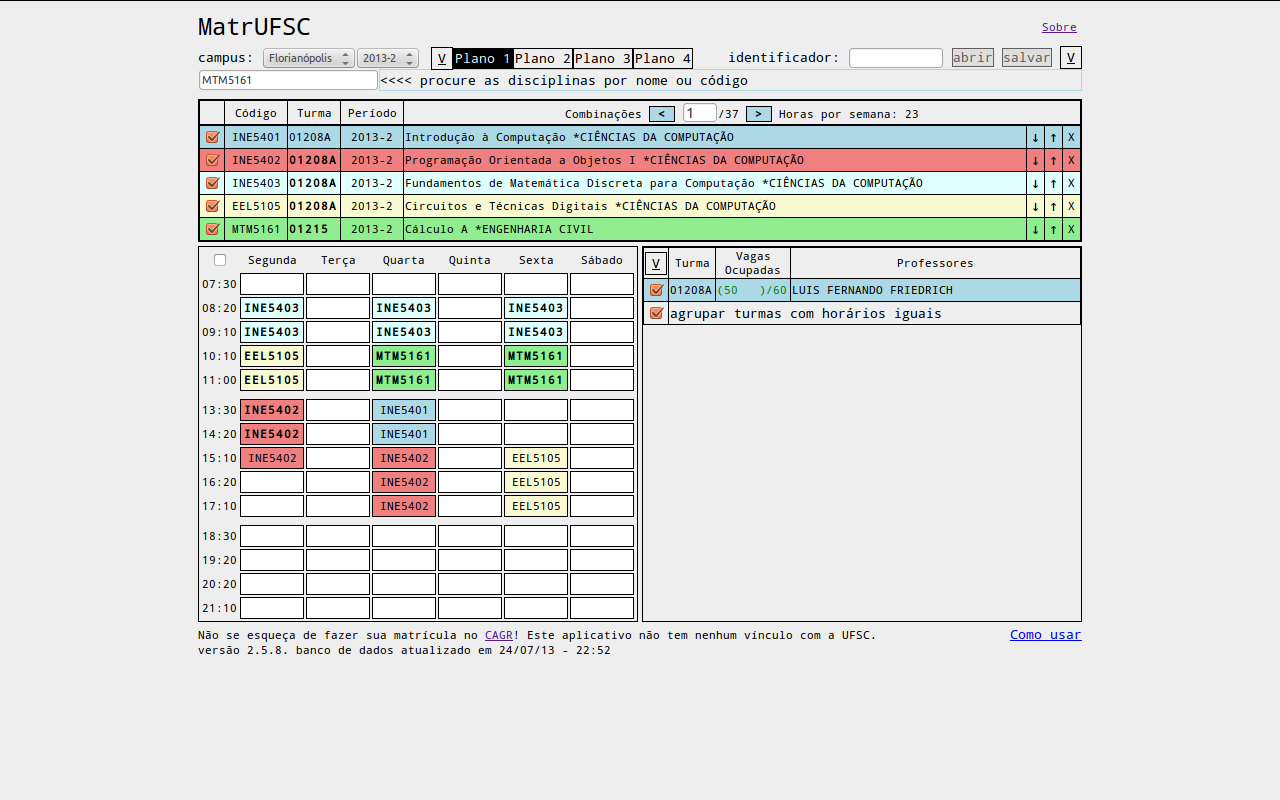
\includegraphics[width=0.99\columnwidth]{matrufsc.png}
		\end{center}
		
		\vskip4ex

%		\definecolor{shadecolor}{named}{treinamento}
%		\begin{shaded}
%		{\footnotesize}
%		\end{shaded}
%
%
%		\definecolor{shadecolor}{named}{reconstrucao}
%		\begin{shaded}
%		{\footnotesize}
%		\end{shaded}

		\end{column}
		\begin{column}{0.28\paperwidth}
			Um sistema que também incorpora uma funcionalidade similar à do MatrUSP,
			apesar de bem mais abrangente, é o \textbf{GDE} \cite{gde}, desenvolvido por Felipe 
			Guaycuru de C. B. Franco e utilizado pelos alunos da Unicamp. O GDE 
			incorpora funcionalidades ainda de rede social, exibe o mapa de pré-requisitos
			das disciplinas do currículo do aluno, informações sobre o restaurante 
			universitário, dentre outros recursos. Atualmente é apoiado pela universidade
			que fornece um \emph{link} para o GDE no sistema de gerenciamento oficial
			da Unicamp.
			
			
			\begin{center}
				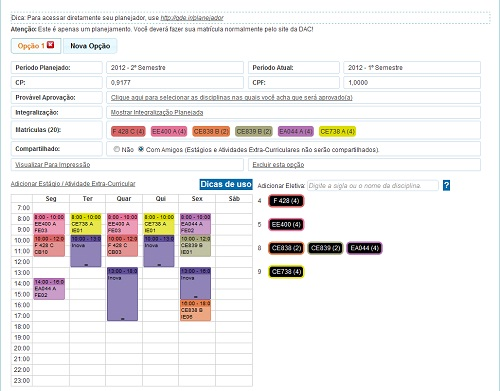
\includegraphics[width=0.99\columnwidth]{gde.jpg}
			\end{center}	
		
%			\hfill{\includegraphics[width=0.8\columnwidth]{figura.pdf}}\\
%			\hfill{\footnotesize{\emph{Descrição minimalista 1}}}
%			\vskip2ex

		\end{column}
		\end{columns}

	\end{block}
	%\vskip2ex

\end{column}
\end{columns}

\vskip2ex

% ---------------------------------------------------------------------------- %

\begin{columns}[t] 
\begin{column}{0.35\paperwidth}

	\begin{block}{Funcionamento}
		O MatrUSP é composto por duas camadas basicamente independentes. A primeira
		reside no servidor do Projeto Apoio BCC e é responsável por fazer o 
		\emph{scraping} dos dados do JupiterWeb diariamente à meia-noite.
		
		\vskip2ex
		
		O trabalho de scraping é feito através de um script Python auxiliado 
		pela biblioteca \emph{BeautifulSoup} para a extração das informações 
		públicas disponíveis no JupiterWeb.
		
		\vskip2ex
		
		O resultado desse processamento é um arquivo JSON que contém uma compilação
		de todas as disciplinas que possuem oferecimento para o próximo semestre
		e com elas todas as turmas disponíveis com seus horários.
		
		\vskip2ex
		
		A segunda camada reside no navegador do usuário e é implementada em 
		JavaScript + HTML + CSS puros. Essa camada é o modelo lógico principal do serviço,
		sendo responsável por receber quais matérias o usuário deseja cursar,
		verificar quais turmas estão disponíveis e gerar todas as combinações 
		possíveis de horários para o usuário.
		
	\end{block}
	
	\vspace{1.0em}

	\begin{block}{MatrUSP na Mídia}
		\begin{itemize}
			\item \textbf{Aluno do IME elabora site para ajudar estudantes na matrícula}
			-- \emph{Jornal do Campus}
			\vskip2ex
			\item Mais de \textbf{1000 likes} no Facebook em três dias
		\end{itemize}
	\end{block}


\end{column}

% ---------------------------------------------------------------------------- %
\begin{column}{0.61\paperwidth} 
\begin{block}{Resultados}
	\begin{center}
		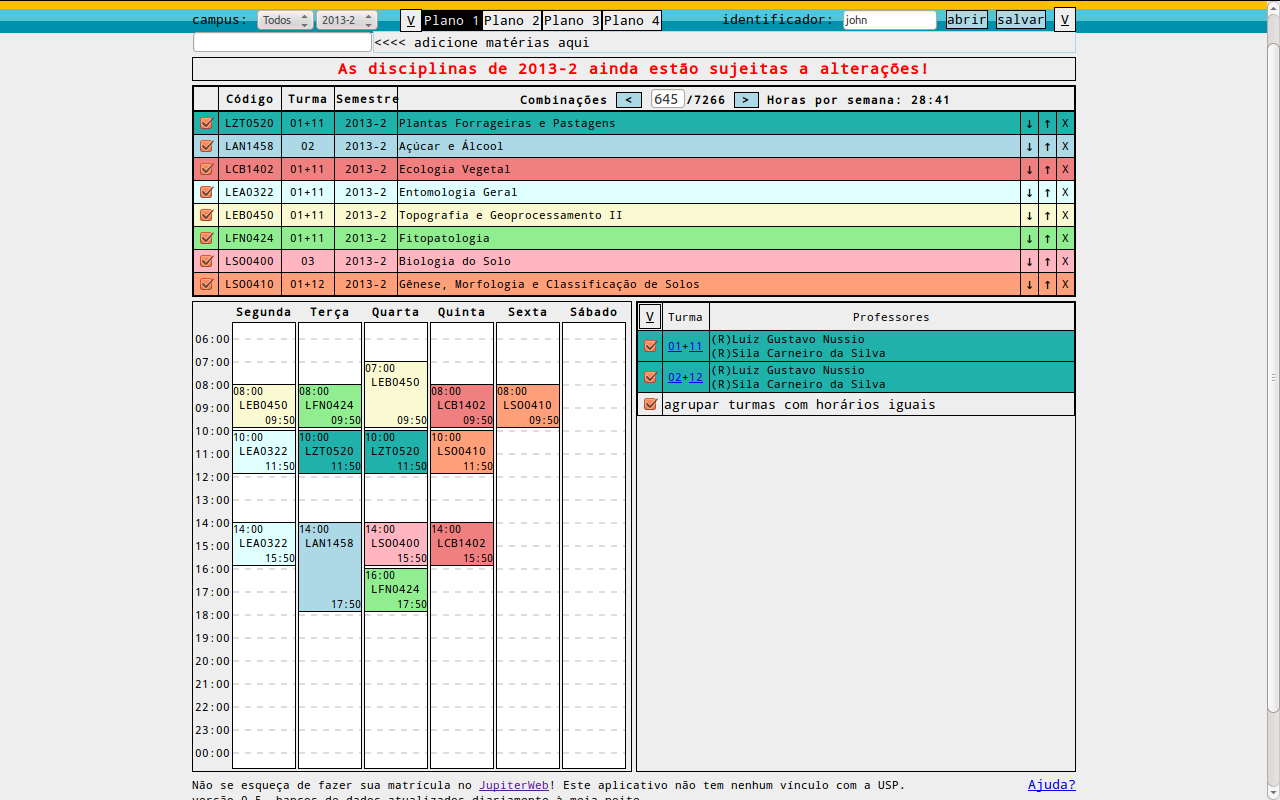
\includegraphics[width=\columnwidth]{matrusp.png}\\
		\hfill\emph{Exemplo: Grade horária de aluno da ESALQ, mais de
		7000 combinações de turmas viáveis}
	\end{center}


\begin{columns}[t] 
	\begin{column}{0.45\columnwidth}
	\end{column}

	\begin{column}{0.45\columnwidth}
	\end{column}
\end{columns}

\vskip2ex


\end{block}

\end{column}
\end{columns}

\begin{columns}[t] 
	\begin{column}{0.35\columnwidth}

		\begin{block}{Agradecimentos}
			O autor gostaria de agradecer a Ramiro Polla pelo código fonte original
			do MatrUFSC e o apoio financeiro da Universidade de São
			Paulo através do programa Ensinar com Pesquisa, que financia o Projeto
			Apoio BCC, do qual o autor é bolsista de iniciação científica.
		\end{block}

	\end{column}

	\begin{column}{0.61\columnwidth}
		\begin{block}{Referências}
			\footnotesize{\begin{thebibliography}{99}
			\bibitem{usp_numeros}
			UNIVERSIDADE DE SÃO PAULO, ``\textbf{USP em Números},'' \emph{Base de dados 2012},
			Disponível em \url{http://www5.usp.br/usp-em-numeros/}. Acesso em 24 de julho de 2013.

			\bibitem{matrufsc}
			R. Polla, ``\textbf{MatrUFSC},'',
			Disponível em \url{http://ramiro.arrozcru.org/matrufsc}. Acesso em 24 de julho de 2013.

			\bibitem{gde}
			F. G. de C. B. Franco , ``\textbf{GDE, a rede de auxílio acadêmico},''
			Disponível em \url{http://grade.daconline.unicamp.br/visoes/Bemvindo.php}. Acesso em 24 de julho de 2013.
			\end{thebibliography}}

		\end{block}
	
	\end{column}
\end{columns}


% ---------------------------------------------------------------------------- %
\end{frame}
\end{document}
